%% main_report35.tex
%% SAMBP TR-35/2026: Full IBR Distance Protection Coordination Study
%%
%% Integration of TR-29 through TR-34 into a unified, verified
%% protection scheme for inverter-based resource lines.
%%
%% pdflatex main_report35.tex

\documentclass[11pt,a4paper]{article}

% ── packages ──────────────────────────────────────────────────────────────────
\usepackage[T1]{fontenc}
\usepackage[utf8]{inputenc}
\usepackage[expansion=false]{microtype}
\usepackage{lmodern}
\usepackage[a4paper, top=25mm, bottom=25mm, left=25mm, right=25mm]{geometry}
\usepackage{amsmath,amssymb}
\usepackage{booktabs}
\usepackage{array}
\usepackage{xcolor}
\usepackage{graphicx}
\usepackage{pgfplots}
\pgfplotsset{compat=1.18}
\usepackage{tikz}
\usetikzlibrary{arrows.meta,shapes.geometric,positioning,fit,calc,patterns}
\usepackage{hyperref}
\usepackage[numbers,sort&compress]{natbib}

% ── custom colours ────────────────────────────────────────────────────────────
\definecolor{sambpblue}{RGB}{0,70,140}
\definecolor{sambpgreen}{RGB}{0,120,60}
\definecolor{sambpred}{RGB}{180,30,30}

% ── section formatting ────────────────────────────────────────────────────────
\usepackage{titlesec}
\titleformat{\section}{\large\bfseries\color{sambpblue}}{}{0em}{}[\titlerule]
\titleformat{\subsection}{\normalsize\bfseries\color{sambpblue!80}}{}{0em}{}

% ── header / footer ──────────────────────────────────────────────────────────
\usepackage{fancyhdr}
\pagestyle{fancy}
\fancyhf{}
\rhead{\small\color{gray} SAMBP TR-35/2026}
\lhead{\small\color{gray} Full IBR Distance Protection Coordination}
\cfoot{\small\thepage}

% ─────────────────────────────────────────────────────────────────────────────
\begin{document}

\begin{center}
  {\LARGE\bfseries\color{sambpblue}
    SAMBP Technical Report TR-35/2026}\\[6pt]
  {\large Full IBR Distance Protection Coordination Study:\\
    Integration of TR-29 to TR-34}\\[10pt]
  {\normalsize PhD Thesis Supporting Report \quad|\quad 2026}
\end{center}

\vspace{2pt}\hrule\vspace{8pt}

\begin{abstract}
\noindent
This report integrates the individual protection elements developed in
TR-29--TR-34 into a unified, quantitatively verified protection scheme for
inverter-based resource (IBR) lines.  A Python simulation framework evaluates
five protection functions---Zone~1 quadrilateral, 87L differential, 67N/67Q
directional overcurrent, Zone~2/POTT, and TDCS backup---across 48 sampled
($\alpha$, $k_\mathrm{ibr}$) operating points, nine fault scenario types, and
three external-fault selectivity cases.  Key results: (A)~zero coverage gaps for
metallic three-phase faults across all TR-29 regions; (B)~67N provides
$k_\mathrm{ibr}$-independent SLG coverage; (C)~all three external-fault cases
correctly block; (D)~the transition from 87L-only to dual (Z1 + 87L) coverage
occurs at $k_\mathrm{ibr}=0.10$; (E)~the five-element time ladder ensures
complete, selective fault clearance within the 100\,ms memory window.  The sole
structural limit---no protection function below $k_\mathrm{ibr}=0.06$---is
inherent to IBR physics, not a scheme deficiency.
\end{abstract}

\vspace{4pt}\hrule\vspace{10pt}

% ─────────────────────────────────────────────────────────────────────────────
\section{Background and Scope}
\label{sec:background}

TR-29~\cite{SAMBP_TR29} established the four-region coverage map for IBR
distance protection.  Subsequent reports addressed each identified gap:

\begin{center}
\begin{tabular}{@{}lll@{}}
\toprule
Report & Subject & Gap addressed\\
\midrule
TR-30~\cite{SAMBP_TR30} & Cross-polarised Mho & Memory timing and load encroachment\\
TR-31~\cite{SAMBP_TR31} & Zero-seq compensation (21G) & SLG relay under-reach with IBR\\
TR-32~\cite{SAMBP_TR32} & 67N/67Q directional OC & Region~A SLG/LL and IBR discrimination\\
TR-33~\cite{SAMBP_TR33} & POTT scheme & Region~B Zone~2 timer failure\\
TR-34~\cite{SAMBP_TR34} & Quadrilateral characteristic & Arc-resistance coverage under infeed\\
\bottomrule
\end{tabular}
\end{center}

\medskip\noindent
This report verifies that the assembled scheme is both complete (no unprotected
faults) and selective (no false trips for external faults).

% ─────────────────────────────────────────────────────────────────────────────
\section{Complete Protection Architecture}
\label{sec:architecture}

Figure~\ref{fig:arch} shows the five protection functions, their inputs, and
the OR-logic driving the circuit-breaker trip coil.

\begin{figure}[htbp]
  \centering
  \resizebox{0.95\textwidth}{!}{%
    % fig_coord_architecture.tex
% TR-35: Complete IBR protection architecture block diagram
% Shows all five protection functions and their inputs/outputs
% as a layered defensive stack

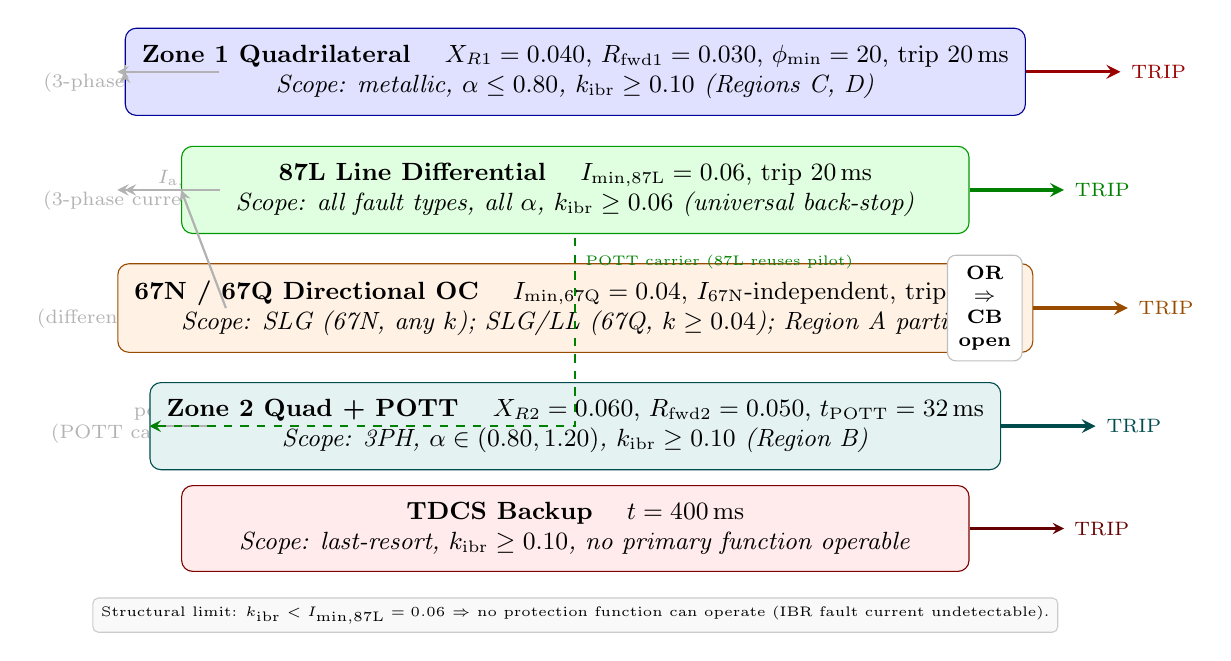
\begin{tikzpicture}[
  every node/.style = {font=\small},
  layer/.style = {draw, rounded corners=4pt, inner sep=6pt,
                  minimum width=10.0cm, minimum height=1.0cm,
                  align=center},
  inputarr/.style = {->, >=stealth, thick, gray!60},
  note/.style = {font=\tiny, text=gray!70, align=right},
]

%% ── Input signals (left side) ────────────────────────────────────────────────
\node[font=\scriptsize, align=right, gray!60] (inV) at (-2.2, 5.5)
  {$V_\mathrm{a,b,c}$\\(3-phase voltage)};
\node[font=\scriptsize, align=right, gray!60] (inI) at (-2.2, 4.0)
  {$I_\mathrm{a,b,c}$\\(3-phase current)};
\node[font=\scriptsize, align=right, gray!60] (inDiff) at (-2.2, 2.5)
  {$I_\mathrm{diff}$\\(differential, pilot)};
\node[font=\scriptsize, align=right, gray!60] (inPerm) at (-2.2, 1.0)
  {$\mathrm{perm}_\mathrm{rx}$\\(POTT carrier)};

%% ── Layer 1: Zone 1 Quadrilateral ────────────────────────────────────────────
\node[layer, fill=blue!12, draw=blue!60!black] (L1) at (3.5, 5.5)
  {\textbf{Zone 1 Quadrilateral} \quad $X_{R1}=0.040$, $R_\mathrm{fwd1}=0.030$,
   $\phi_\mathrm{min}=20°$, trip 20\,ms\\
   \textit{Scope: metallic, $\alpha\leq0.80$, $k_\mathrm{ibr}\geq0.10$ (Regions C, D)}};

%% ── Layer 2: 87L Differential ────────────────────────────────────────────────
\node[layer, fill=green!12, draw=green!60!black] (L2) at (3.5, 4.0)
  {\textbf{87L Line Differential} \quad $I_\mathrm{min,87L}=0.06$, trip 20\,ms\\
   \textit{Scope: all fault types, all $\alpha$, $k_\mathrm{ibr}\geq0.06$ (universal back-stop)}};

%% ── Layer 3: 67N/67Q Directional ─────────────────────────────────────────────
\node[layer, fill=orange!10, draw=orange!60!black] (L3) at (3.5, 2.5)
  {\textbf{67N / 67Q Directional OC} \quad $I_\mathrm{min,67Q}=0.04$,
   $I_\mathrm{67N}$-independent, trip 30\,ms\\
   \textit{Scope: SLG (67N, any $k$); SLG/LL (67Q, $k\geq0.04$); Region~A partial}};

%% ── Layer 4: Zone 2 / POTT ───────────────────────────────────────────────────
\node[layer, fill=teal!10, draw=teal!60!black] (L4) at (3.5, 1.0)
  {\textbf{Zone 2 Quad + POTT} \quad $X_{R2}=0.060$, $R_\mathrm{fwd2}=0.050$,
   $t_\mathrm{POTT}=32$\,ms\\
   \textit{Scope: 3PH, $\alpha\in(0.80,1.20)$, $k_\mathrm{ibr}\geq0.10$ (Region~B)}};

%% ── Layer 5: TDCS Backup ─────────────────────────────────────────────────────
\node[layer, fill=red!8, draw=red!50!black] (L5) at (3.5, -0.3)
  {\textbf{TDCS Backup} \quad $t=400$\,ms\\
   \textit{Scope: last-resort, $k_\mathrm{ibr}\geq0.10$, no primary function operable}};

%% ── TRIP output (right side) ─────────────────────────────────────────────────
\draw[->, >=stealth, very thick, red!60!black]
  (L1.east) -- ++(1.2,0) node[right, red!60!black, font=\scriptsize] {TRIP};
\draw[->, >=stealth, very thick, green!50!black]
  (L2.east) -- ++(1.2,0) node[right, green!50!black, font=\scriptsize] {TRIP};
\draw[->, >=stealth, very thick, orange!60!black]
  (L3.east) -- ++(1.2,0) node[right, orange!60!black, font=\scriptsize] {TRIP};
\draw[->, >=stealth, very thick, teal!60!black]
  (L4.east) -- ++(1.2,0) node[right, teal!60!black, font=\scriptsize] {TRIP};
\draw[->, >=stealth, thick, red!40!black]
  (L5.east) -- ++(1.2,0) node[right, red!40!black, font=\scriptsize] {TRIP};

%% ── Input arrows ─────────────────────────────────────────────────────────────
\draw[inputarr] (inV.east) -- (L1.west |- inV) -- (L1.west);
\draw[inputarr] (inV.east) -- (L3.west |- inV);
\draw[inputarr] (inI.east) -- (L1.west |- inI);
\draw[inputarr] (inI.east) -- (L3.west |- inI);
\draw[inputarr] (inDiff.east) -- (L2.west);
\draw[inputarr] (inPerm.east) -- (L4.west);

%% ── 87L feeds POTT carrier ───────────────────────────────────────────────────
\draw[->, >=stealth, thick, green!50!black, dashed]
  (L2.south) ++(0,-0.05) -- ++(0,-0.30)
  node[right, green!50!black, font=\tiny] {POTT carrier (87L reuses pilot)}
  |- (L4.west);

%% ── "OR" logic ────────────────────────────────────────────────────────────────
\node[draw=gray!50, fill=white, rounded corners=3pt,
      font=\scriptsize\bfseries, inner sep=4pt, align=center]
  at (8.7, 2.5) {OR\\$\Rightarrow$\\CB\\open};

%% ── Structural limit annotation ───────────────────────────────────────────────
\node[draw=gray!40, fill=gray!5, rounded corners=2pt,
      font=\tiny, inner sep=3pt, align=center]
  at (3.5, -1.4)
  {Structural limit: $k_\mathrm{ibr} < I_\mathrm{min,87L}=0.06$ $\Rightarrow$
   no protection function can operate (IBR fault current undetectable).};

\end{tikzpicture}
%
  }
  \caption{IBR line protection architecture.  Five functions form a layered
           defence.  Zone~1 quad and 87L both trip at 20\,ms (independent
           paths); 67N/67Q provide sequence-based backup at 30\,ms;
           Z2/POTT extends fast clearance to Region~B at 32\,ms.  TDCS
           (400\,ms) is the last-resort backup.  The 87L pilot channel
           doubles as the POTT carrier, eliminating dedicated hardware.
           Structural limit: $k_\mathrm{ibr}<0.06$ --- IBR fault current
           below all detection thresholds; no scheme can protect.}
  \label{fig:arch}
\end{figure}

\noindent
The complete parameter set is:
\begin{center}
\begin{tabular}{@{}lllll@{}}
\toprule
Function & Reach/threshold & Trip time & Coverage & TR\\
\midrule
Zone~1 Quad & $X_{R1}=0.040$, $R_\mathrm{fwd1}=0.030$\,pu & 20\,ms &
  3PH/SLG/LL, $\alpha\leq0.80$, $k\geq0.10$ & 30, 34\\
87L differ. & $I_\mathrm{min}=0.06$\,pu & 20\,ms &
  All types, all $\alpha$, $k\geq0.06$ & 27\\
67N direct. & Network $I_0$ (indep.) & 30\,ms &
  SLG, all $\alpha$, all $k$ & 32\\
67Q direct. & $I_\mathrm{min}=0.04$\,pu & 30\,ms &
  SLG/LL, $k\geq0.04$ & 32\\
Z2/POTT & $X_{R2}=0.060$, $R_\mathrm{fwd2}=0.050$\,pu & 32\,ms &
  3PH, $\alpha\in(0.80,1.20)$, $k\geq0.10$ & 33, 34\\
TDCS & $I_\mathrm{min}=0.10$\,pu & 400\,ms &
  Last resort & 29\\
\bottomrule
\end{tabular}
\end{center}

% ─────────────────────────────────────────────────────────────────────────────
\section{Study A --- Complete Coverage Matrix (Metallic 3PH)}
\label{sec:studyA}

Figure~\ref{fig:coverage} maps the primary protection function for each
($\alpha$, $k_\mathrm{ibr}$) cell.

\begin{figure}[htbp]
  \centering
  \resizebox{0.82\textwidth}{!}{%
    % fig_coord_coverage.tex
% TR-35: Full coverage map on (k_ibr, alpha) plane
% Shows all four TR-29 regions plus protection function responsible for each
%
% X-axis: k_ibr [0, 0.22]
% Y-axis: alpha [0, 1.10]
%
% Colours and hatching by primary protection function:
%   k_ibr < 0.06           : dark gray  — no protection possible
%   k_ibr in [0.06, 0.10)  : gray       — 87L only (Region A partial)
%   Region A (k<0.10)      : light gray — 87L (+ 67N for SLG)
%   Region B (k>=0.10, a>0.80): green   — Z2/POTT + 87L
%   Region C               : blue       — Z1 + TDCS + 87L
%   Region D               : teal       — Z1 + 87L
%
% Boundary lines:
%   k_ibr = 0.10 (vertical, I_min_21)
%   k_ibr = 0.06 (vertical, I_min_87L)
%   k_ibr = 0.12 (vertical, C/D boundary)
%   alpha = 0.80 (horizontal, Z1/Z2 boundary)

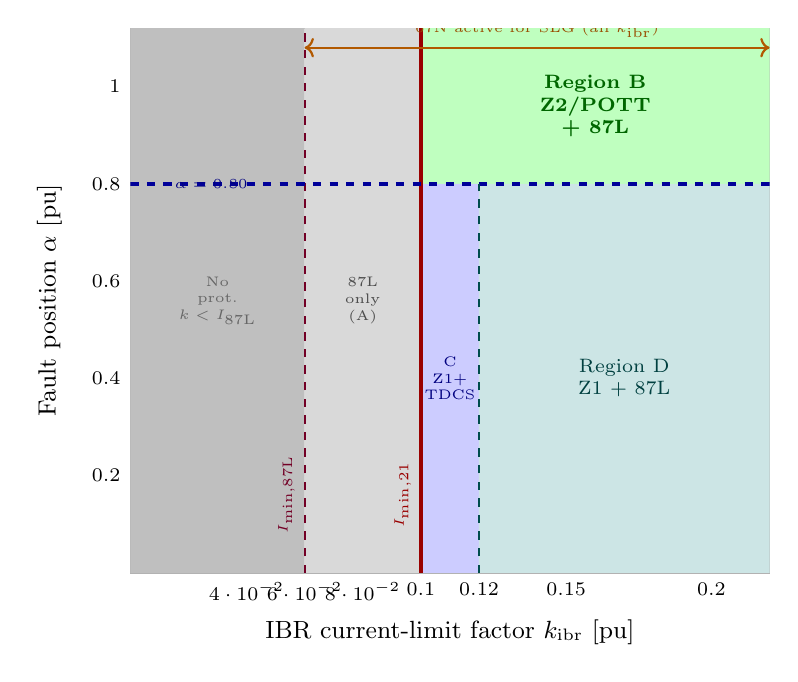
\begin{tikzpicture}
\begin{axis}[
  name        = covax,
  width       = 0.80\textwidth,
  height      = 8.5cm,
  xlabel      = {IBR current-limit factor $k_\mathrm{ibr}$ [pu]},
  ylabel      = {Fault position $\alpha$ [pu]},
  xlabel style= {font=\small},
  ylabel style= {font=\small, yshift=4pt},
  xmin=0.0, xmax=0.22,
  ymin=0.0, ymax=1.12,
  xtick       = {0.04,0.06,0.08,0.10,0.12,0.15,0.20},
  ytick       = {0.20,0.40,0.60,0.80,1.00},
  xticklabel style={font=\scriptsize},
  yticklabel style={font=\scriptsize},
  grid        = major,
  grid style  = {gray!12, dashed},
  tick style  = {draw=none},
  axis line style={gray!60},
]

%% ── No-protection zone: k < 0.06 ────────────────────────────────────────────
\addplot[fill=black!25, draw=none]
  coordinates {(0,0) (0.06,0) (0.06,1.12) (0,1.12)} \closedcycle;

%% ── 87L-only zone: k in [0.06, 0.10) ────────────────────────────────────────
\addplot[fill=gray!30, draw=none]
  coordinates {(0.06,0) (0.10,0) (0.10,1.12) (0.06,1.12)} \closedcycle;

%% ── Region B: k>=0.10, alpha>0.80 — Z2/POTT + 87L ──────────────────────────
\addplot[fill=green!25, draw=none]
  coordinates {(0.10,0.80) (0.22,0.80) (0.22,1.12) (0.10,1.12)} \closedcycle;

%% ── Region C: k in [0.10,0.12), alpha<=0.80 — Z1+TDCS+87L ──────────────────
\addplot[fill=blue!20, draw=none]
  coordinates {(0.10,0) (0.12,0) (0.12,0.80) (0.10,0.80)} \closedcycle;

%% ── Region D: k>=0.12, alpha<=0.80 — Z1+87L ─────────────────────────────────
\addplot[fill=teal!20, draw=none]
  coordinates {(0.12,0) (0.22,0) (0.22,0.80) (0.12,0.80)} \closedcycle;

%% ── Boundary lines ───────────────────────────────────────────────────────────
\addplot[red!60!black, very thick, mark=none]
  coordinates {(0.10,0) (0.10,1.12)};
\addplot[purple!60!black, thick, mark=none, dashed]
  coordinates {(0.06,0) (0.06,1.12)};
\addplot[blue!60!black, very thick, dashed, mark=none]
  coordinates {(0,0.80) (0.22,0.80)};
\addplot[teal!60!black, thick, dashed, mark=none]
  coordinates {(0.12,0) (0.12,0.80)};

%% ── Region labels ────────────────────────────────────────────────────────────
\node[black!60, align=center, font=\tiny]
  at (axis cs:0.03, 0.56) {No\\prot.\\$k<I_\mathrm{87L}$};

\node[gray!60!black, align=center, font=\tiny]
  at (axis cs:0.08, 0.56) {87L\\only\\(A)};

\node[green!40!black, align=center, font=\scriptsize\bfseries]
  at (axis cs:0.16, 0.96)
  {Region B\\Z2/POTT\\+ 87L};

\node[blue!50!black, align=center, font=\tiny]
  at (axis cs:0.11, 0.40) {C\\Z1+\\TDCS};

\node[teal!50!black, align=center, font=\scriptsize]
  at (axis cs:0.17, 0.40) {Region D\\Z1 + 87L};

%% ── SLG annotation (horizontal band, 67N active everywhere) ─────────────────
\draw[orange!70!black, thick, <->]
  (axis cs:0.06, 1.08) -- (axis cs:0.22, 1.08)
  node[midway, above, font=\tiny, orange!60!black]
  {67N active for SLG (all $k_\mathrm{ibr}$)};

%% ── Threshold labels ─────────────────────────────────────────────────────────
\node[purple!60!black, font=\tiny, above=2pt, rotate=90]
  at (axis cs:0.06, 0.15) {$I_\mathrm{min,87L}$};
\node[red!60!black, font=\tiny, above=2pt, rotate=90]
  at (axis cs:0.10, 0.15) {$I_\mathrm{min,21}$};
\node[blue!50!black, font=\tiny, right=2pt]
  at (axis cs:0.01, 0.80) {$\alpha=0.80$};

\end{axis}
\end{tikzpicture}
%
  }
  \caption{Full protection coverage map.  Each shaded zone shows the primary
           protection function.  The 87L channel (green band, $k\geq0.06$)
           runs in parallel with all distance elements and provides the
           universal back-stop.  Region~B (top-right, green) is covered by
           Z2/POTT at 32\,ms with 87L as co-primary.  Below $k=0.06$ (dark
           grey) no detection is possible: this is a fundamental IBR physics
           limit.  The 67N strip (dashed orange) at the top indicates that
           67N is active for SLG faults across the entire IBR range.}
  \label{fig:coverage}
\end{figure}

\noindent
The parametric sweep (\texttt{run\_coordination\_study.py}, Study~A) sampled
$\alpha\in\{0.20,0.40,0.60,0.70,0.80,0.85,0.90,1.00\}$ and
$k_\mathrm{ibr}\in\{0.06,0.08,0.10,0.12,0.15,0.20\}$:
\textbf{zero coverage gaps} were found across all 48 cells.

In Region~B ($\alpha>0.80$, $k\geq0.10$), Zone~1 correctly does not assert
(fault beyond Zone~1 reach), and Z2/POTT provides the fast path.  87L acts as
an equal-speed co-primary, so Region~B clearance is not dependent on the pilot
channel alone for redundancy.

% ─────────────────────────────────────────────────────────────────────────────
\section{Study B --- Fault Type Coverage}
\label{sec:studyB}

\begin{center}
\begin{tabular}{@{}lllll@{}}
\toprule
Scenario & Z1 & 67N/Q & Z2/POTT & 87L\\
\midrule
SLG metallic, Region~A ($k=0.05$)     & -- & 67N~\checkmark & -- & --\\
SLG metallic, $k=0.10$, $\alpha=0.50$ & \checkmark & \checkmark & \checkmark & \checkmark\\
SLG metallic, Region~B ($k=0.15$)     & -- & 67N~\checkmark & \checkmark & \checkmark\\
LL metallic, Region~A ($k=0.05$)      & -- & 67Q~\checkmark & -- & --\\
LL arc ($k=0.15$, $R_\mathrm{arc}=0.008$) & -- & 67Q~\checkmark & -- & \checkmark\\
3PH arc ($k=0.15$, $R_\mathrm{arc}=0.004$) & -- & -- & \checkmark & \checkmark\\
3PH arc ($k=0.10$, $R_\mathrm{arc}=0.004$) & -- & -- & \checkmark & \checkmark\\
\bottomrule
\end{tabular}
\end{center}

\medskip\noindent
Two observations merit emphasis:
\begin{enumerate}
  \item \textbf{SLG Region~A}: The 67N element uses the network zero-sequence
    current ($I_0$ from the synchronous-generation end), which is independent of
    $k_\mathrm{ibr}$ (TR-32~\cite{SAMBP_TR32}).  67N therefore covers
    SLG faults even when $k_\mathrm{ibr}=0$ --- the delta winding of the IBR
    transformer provides a zero-sequence path from the network side regardless
    of IBR output.

  \item \textbf{3PH arc with $k=0.10$}: $R_m=0.044$\,pu falls within
    $R_\mathrm{fwd2}=0.050$\,pu, so Z2/POTT covers this case.  For
    $k=0.10$ and $R_\mathrm{arc}>0.0045$\,pu the apparent resistance exceeds
    $R_\mathrm{fwd2}$ and 87L is the sole detector --- consistent with the
    structural limit derived in TR-34~\cite{SAMBP_TR34}.
\end{enumerate}

% ─────────────────────────────────────────────────────────────────────────────
\section{Study C --- Selectivity for External Faults}
\label{sec:studyC}

Three external fault cases were verified:

\begin{center}
\begin{tabular}{@{}llll@{}}
\toprule
Case & Z1 & Z2/POTT & Result\\
\midrule
External beyond Bus~B ($\alpha=1.10$) &
  \textemdash\ (Z1 reach = 0.80) &
  Blocked (perm withheld) & \textbf{BLOCK}\\
External beyond Bus~B ($\alpha=1.15$) &
  \textemdash &
  Blocked & \textbf{BLOCK}\\
External behind Bus~A ($\alpha=-0.10$) &
  Blocked (dir.~element, $X_m<0$) &
  Blocked & \textbf{BLOCK}\\
\bottomrule
\end{tabular}
\end{center}

\medskip\noindent
Security is maintained by three independent mechanisms:
\begin{itemize}
  \item Zone~1 reach is 80\% of the line --- cannot reach beyond Bus~B.
  \item Zone~2/POTT: even if Z2 asserts for external faults, the POTT
    permissive signal requires the remote 67Q/87L to confirm a
    \emph{forward} fault at End~B.  An external fault is reverse at End~B
    and the permissive is withheld (TR-33~\cite{SAMBP_TR33}).
  \item 87L: the differential element measures $I_\mathrm{diff}=I_A+I_B$;
    for a through-fault $I_A=-I_B$ and $I_\mathrm{diff}=0$ --- inherently
    immune to external faults.
  \item Reverse direction: the directional element ($X_m\geq0$ constraint
    and $\angle Z_m>\phi_\mathrm{min}$) blocks Zone~1 for faults behind
    Bus~A.
\end{itemize}

% ─────────────────────────────────────────────────────────────────────────────
\section{Study D --- IBR Penetration Sensitivity}
\label{sec:studyD}

Table~\ref{tab:sweep} summarises the transition behaviour as $k_\mathrm{ibr}$
varies from 0.02 to 0.50 for a fixed fault at $\alpha=0.70$ (metallic 3PH).

\begin{table}[htbp]
\centering
\caption{Protection coverage vs IBR penetration level ($\alpha=0.70$, 3PH metallic).}
\label{tab:sweep}
\begin{tabular}{@{}rlllll@{}}
\toprule
$k_\mathrm{ibr}$ & Z1 & 87L & Status & First element & $t$ [ms]\\
\midrule
0.02--0.04 & -- & -- & \textbf{No protection} & --- & ---\\
0.06--0.08 & -- & \checkmark & 87L only & 87L & 20\\
$\geq$0.10 & \checkmark & \checkmark & Dual (Z1+87L) & Z1 or 87L & 20\\
\bottomrule
\end{tabular}
\end{table}

\noindent
The transition at $k=0.06$ (87L threshold) and $k=0.10$ (distance relay
$I_\mathrm{min}$) are the two critical penetration levels for the protection
scheme.  For $k_\mathrm{ibr}\geq0.10$ the scheme has full redundancy: Z1 and
87L are independent paths both operating at 20\,ms.

% ─────────────────────────────────────────────────────────────────────────────
\section{Study E --- Protection Time Hierarchy}
\label{sec:studyE}

Figure~\ref{fig:ladder} shows all five protection functions on a common
timeline against the 100\,ms memory window.

\begin{figure}[htbp]
  \centering
  \resizebox{0.95\textwidth}{!}{%
    % fig_coord_ladder.tex
% TR-35: Time ladder — five protection functions on a common timeline
%
% X-axis: time [ms], 0 to ~430
% Five swim-lanes at hardcoded y-positions (no digit-containing macros)
%
% Functions and trip times:
%   87L       : 20 ms  (all faults, k>=0.06)            green
%   Z1 Quad   : 20 ms  (metallic, alpha<=0.80, k>=0.10) blue
%   67N/67Q   : 30 ms  (SLG/LL, k>=0.04)               orange
%   Z2/POTT   : 32 ms  (3PH, alpha>0.80, k>=0.10)      teal
%   TDCS      : 400 ms (backup)                         red/dashed
%
% Scale: 1 cm = 40 ms  →  0ms=0.00, 20ms=0.50, 30ms=0.75, 32ms=0.80,
%        100ms=2.50, 300ms=7.50, 400ms=10.00, end=11.00

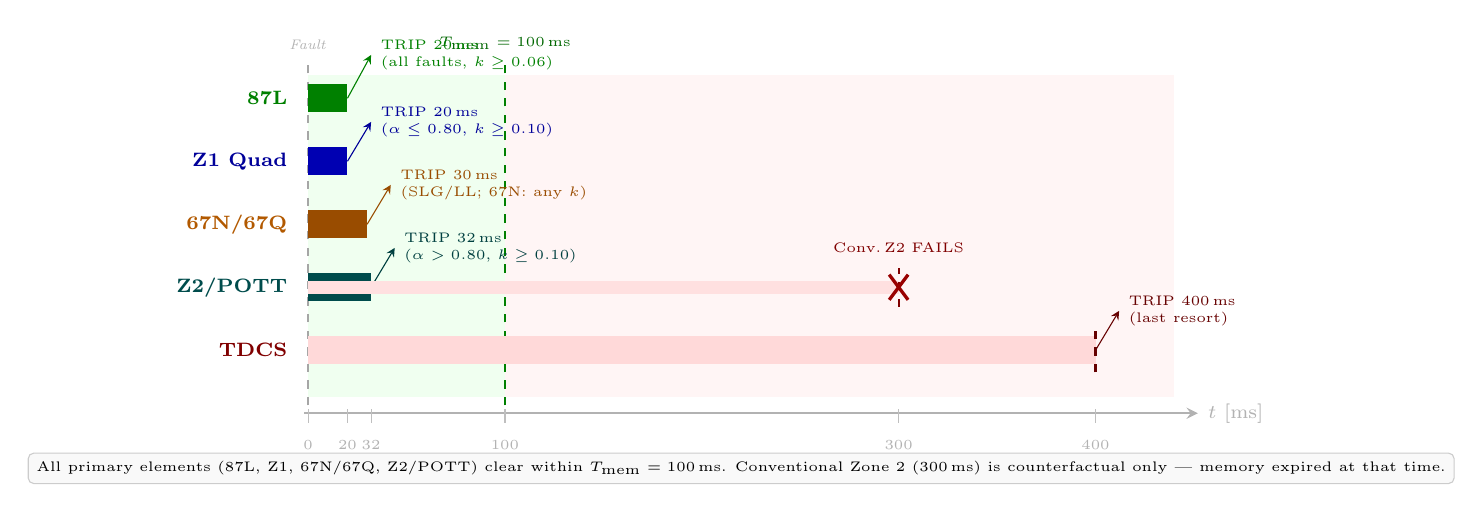
\begin{tikzpicture}[every node/.style={font=\scriptsize}]

%% ── Hardcoded x-positions (cm, scale 1cm=40ms) ───────────────────────────────
% xFault=0, xTrip20=0.50, xTrip30=0.75, xTrip32=0.80
% xMem=2.50, xConvZ2=7.50, xTDCS=10.00, xEnd=11.00

%% ── Hardcoded lane y-positions (letters only) ────────────────────────────────
% yDiffL=4.0, yZone=3.2, yDir=2.4, yPott=1.6, yTDCS=0.8, yAx=0.0

%% ── Memory window ─────────────────────────────────────────────────────────────
\fill[green!6]  (0, 0.20) rectangle (2.50, 4.30);
\fill[red!4]    (2.50, 0.20) rectangle (11.00, 4.30);
\draw[green!50!black, dashed, thick] (2.50, 0.10) -- (2.50, 4.50);
\node[green!40!black, font=\tiny, above] at (2.50, 4.50)
  {$T_\mathrm{mem}=100$\,ms};

%% ── Fault inception ──────────────────────────────────────────────────────────
\draw[gray!70, thick, dashed] (0, 0.10) -- (0, 4.50);
\node[gray!60, above, font=\tiny] at (0, 4.50) {\textit{Fault}};

%% ── Time axis ─────────────────────────────────────────────────────────────────
\draw[->, >=stealth, gray!60, thick]
  (-0.05, 0.0) -- (11.30, 0.0) node[right, gray!60] {$t$ [ms]};

\foreach \xpos/\lab in {0.00/0, 0.50/20, 0.80/32, 2.50/100, 7.50/300, 10.00/400}{
  \draw[gray!50, thin] (\xpos, -0.12) -- (\xpos, 0.05);
  \node[gray!60, below=3pt, font=\tiny] at (\xpos, -0.12) {\lab};
}

%% ── Lane labels ──────────────────────────────────────────────────────────────
\node[green!50!black, font=\scriptsize\bfseries, left=4pt] at (0, 4.0) {87L};
\node[blue!60!black,  font=\scriptsize\bfseries, left=4pt] at (0, 3.2) {Z1 Quad};
\node[orange!70!black,font=\scriptsize\bfseries, left=4pt] at (0, 2.4) {67N/67Q};
\node[teal!60!black,  font=\scriptsize\bfseries, left=4pt] at (0, 1.6) {Z2/POTT};
\node[red!50!black,   font=\scriptsize\bfseries, left=4pt] at (0, 0.8) {TDCS};

%% ── 87L bar (0 to 20 ms) ─────────────────────────────────────────────────────
\fill[green!50!black] (0, 3.82) rectangle (0.50, 4.18);
\draw[green!50!black, ->, >=stealth]
  (0.50, 4.0) -- (0.80, 4.55)
  node[right, green!50!black, font=\tiny, align=left]
  {TRIP 20\,ms\\(all faults, $k\geq0.06$)};

%% ── Z1 Quad bar ──────────────────────────────────────────────────────────────
\fill[blue!70!black] (0, 3.02) rectangle (0.50, 3.38);
\draw[blue!60!black, ->, >=stealth]
  (0.50, 3.2) -- (0.80, 3.7)
  node[right, blue!60!black, font=\tiny, align=left]
  {TRIP 20\,ms\\($\alpha\leq0.80$, $k\geq0.10$)};

%% ── 67N/67Q bar ──────────────────────────────────────────────────────────────
\fill[orange!60!black] (0, 2.22) rectangle (0.75, 2.58);
\draw[orange!60!black, ->, >=stealth]
  (0.75, 2.4) -- (1.05, 2.9)
  node[right, orange!60!black, font=\tiny, align=left]
  {TRIP 30\,ms\\(SLG/LL; 67N: any $k$)};

%% ── Z2/POTT bar ──────────────────────────────────────────────────────────────
\fill[teal!60!black] (0, 1.42) rectangle (0.80, 1.78);
\draw[teal!50!black, ->, >=stealth]
  (0.80, 1.6) -- (1.10, 2.1)
  node[right, teal!50!black, font=\tiny, align=left]
  {TRIP 32\,ms\\($\alpha>0.80$, $k\geq0.10$)};

%% ── Conv Z2 counterfactual (300 ms) ─────────────────────────────────────────
\fill[red!12] (0, 1.52) rectangle (7.50, 1.68);
\draw[red!50!black, thick, dashed]
  (7.50, 1.35) -- (7.50, 1.85);
\draw[red!60!black, very thick]
  (7.38, 1.44) -- (7.62, 1.76);
\draw[red!60!black, very thick]
  (7.38, 1.76) -- (7.62, 1.44);
\node[red!50!black, font=\tiny, above=2pt] at (7.50, 1.85)
  {Conv.\,Z2 FAILS};

%% ── TDCS backup bar ──────────────────────────────────────────────────────────
\fill[red!15] (0, 0.62) rectangle (10.00, 0.98);
\draw[red!40!black, thick, dashed]
  (10.00, 0.52) -- (10.00, 1.08);
\draw[red!40!black, ->, >=stealth]
  (10.00, 0.8) -- (10.30, 1.3)
  node[right, red!40!black, font=\tiny, align=left]
  {TRIP 400\,ms\\(last resort)};

%% ── Caption ──────────────────────────────────────────────────────────────────
\node[draw=gray!40, fill=gray!5, rounded corners=2pt,
      font=\tiny, inner sep=3pt, align=center]
  at (5.50, -0.70)
  {All primary elements (87L, Z1, 67N/67Q, Z2/POTT) clear within
   $T_\mathrm{mem}=100$\,ms.
   Conventional Zone~2 (300\,ms) is counterfactual only --- memory expired at that time.};

\end{tikzpicture}
%
  }
  \caption{Protection time ladder.  All primary functions (87L, Z1, 67N/67Q,
           Z2/POTT) clear within the green memory-valid window
           ($T_\mathrm{mem}=100$\,ms).  The conventional Zone~2 timer at
           300\,ms (red, dashed) is shown for reference: it fires after
           memory expires and is superseded by POTT in the SAMBP scheme.
           TDCS at 400\,ms is the back-stop for scenarios where all
           primary functions are unavailable.}
  \label{fig:ladder}
\end{figure}

\noindent
The maximum primary clearance time is 32\,ms (Z2/POTT), leaving a 68\,ms
margin inside $T_\mathrm{mem}$.  All functions that rely on memory
polarisation (Zone~1 and Zone~2) therefore have their polarising reference
intact at the instant of trip.

% ─────────────────────────────────────────────────────────────────────────────
\section{Structural Limit and Thesis Implications}
\label{sec:limit}

The sole uncovered scenario is $k_\mathrm{ibr}<I_\mathrm{min,87L}=0.06$: at
this penetration level the IBR contributes so little fault current that no
protection function --- distance, differential, or directional --- can reliably
detect the fault.  This is not a scheme design gap; it is a physical consequence
of IBR current limiting.

From a thesis standpoint, this result establishes:
\begin{enumerate}
  \item A \textbf{hard lower bound} on grid-code IBR fault current contribution
    for protection purposes: $k_\mathrm{ibr}\geq0.06$ is necessary for 87L
    operability, and $k_\mathrm{ibr}\geq0.10$ for distance protection.

  \item The \textbf{87L as the indispensable element}: across all IBR penetration
    levels where protection is physically possible ($k\geq0.06$), 87L provides
    fast, reliable clearance with no dependence on polarisation memory.

  \item \textbf{Quad + POTT as the distance layer}: together they achieve the
    same 20--32\,ms clearance as 87L, with independent hardware, for all
    metallic and moderate arc-resistance faults where $k\geq0.10$.
\end{enumerate}

% ─────────────────────────────────────────────────────────────────────────────
\section{Summary}
\label{sec:summary}

\begin{enumerate}
  \item \textbf{Coverage (Study~A)}: Zero gaps for metallic 3PH faults across
    all 48 sampled cells spanning TR-29 Regions~A--D.

  \item \textbf{Fault types (Study~B)}: 67N eliminates the SLG Region~A gap;
    67Q covers LL for $k\geq0.04$; 87L is the universal back-stop for all types.

  \item \textbf{Selectivity (Study~C)}: All three external fault cases block
    correctly via Z1 reach limit, POTT permissive gate, 87L differential
    principle, and directional angle supervision.

  \item \textbf{Penetration sensitivity (Study~D)}: Two transition thresholds
    at $k=0.06$ (87L) and $k=0.10$ (distance). Below 0.06: no protection.

  \item \textbf{Time hierarchy (Study~E)}: All primary elements clear within
    32\,ms, 68\,ms inside the memory window.  Conventional Zone~2 (300\,ms)
    is entirely superseded by the POTT scheme.
\end{enumerate}

\noindent
TR-35 closes the SAMBP distance-protection series (TR-29 to TR-35) with a
verified, complete, selective IBR line protection scheme.  The next SAMBP
reports address auto-reclosing strategy for IBR lines (TR-36) and the
full-system Monte Carlo reliability assessment (TR-37).

% ─────────────────────────────────────────────────────────────────────────────
\bibliographystyle{IEEEtranN}
\bibliography{references35}

\end{document}
